\section{Risultati ottenuti}
\subsection{Metriche utilizzate per singole immagini}
Nell'ambito della computer vision vengono tipicamente utilizzate due tipi di metriche per misurare due diverse proprietà:
\begin{itemize}
\item Corretta determinazione della posizione degli oggetti;
\item Rilevamento l'esistenza degli oggetti nell'immagine e la loro corretta classificazione.
\end{itemize}
Le metriche utilizzate per misurare la bontà dei risultati del progetto sono AP (Average Precision) e mAp (mean Average Precision) le quali misurano la seconda proprietà sopra elencata.
Prima di iniziare a descrivere le due metriche è necessario definire tre concetti che saranno poi coinvolti per il calcolo dei valori delle metriche.
\subsubsection{Precision}
La precision misura l'accuratezza delle classificazioni ed indica la percentuale di classificazioni corrette sulla base di quelle totali e viene calcolata come:
\[
    precision = \frac{TP}{TP + FP}
\]
Dove TP (True Positives) è il numero di classificazioni corrette e FP (False Positives) è il numero di classificazioni errate. E' da sottolineare che se uno stesso elemento viene individuato più di una volta, solo la prima volta conterà come TP mentre il resto delle volte conterà come FP. Questa metrica fornisce un'idea sulla correttezza dei risultati.
\subsubsection{Recall}
La recall misura quanti oggetti sono stati individuati e classificati correttamente sulla base degli oggetti totali, viene calcolata come:
\[
    precision = \frac{TP}{TP + FN}
\]
Dove TP (True Positives) è sempre il numero di classificazioni corrette mentre FN (False Negatives) è il numero di di oggetti che non sono stati individuati ma che se sarebbero stato corretto individuare. Questa metrica fornisce un'idea sulla completezza dei risultati.
\subsubsection{Intersection over union}
L'intersection over union (IoU) misura il grado di sovrapposizione tra due aree e viene usato per misuare il grado di sovrapposizione tra la box dell'oggetto individuato e la box dell'oggetto reale. Viene calcolata come:
\[
    IoU = \frac{AI}{AU}
\]
Dove AI (Area dell'Intersezione) corrisponde all'area dell'intersezione tra le due box e AU (Area dell'Unione) corrisponde all'area dell'unione tra le due box.
Una label per essere considerata come corretta deve avere un valore di IoU maggiore di una soglia stabilità (per esempio 0.5).
\begin{figure}[H]
	\centering
	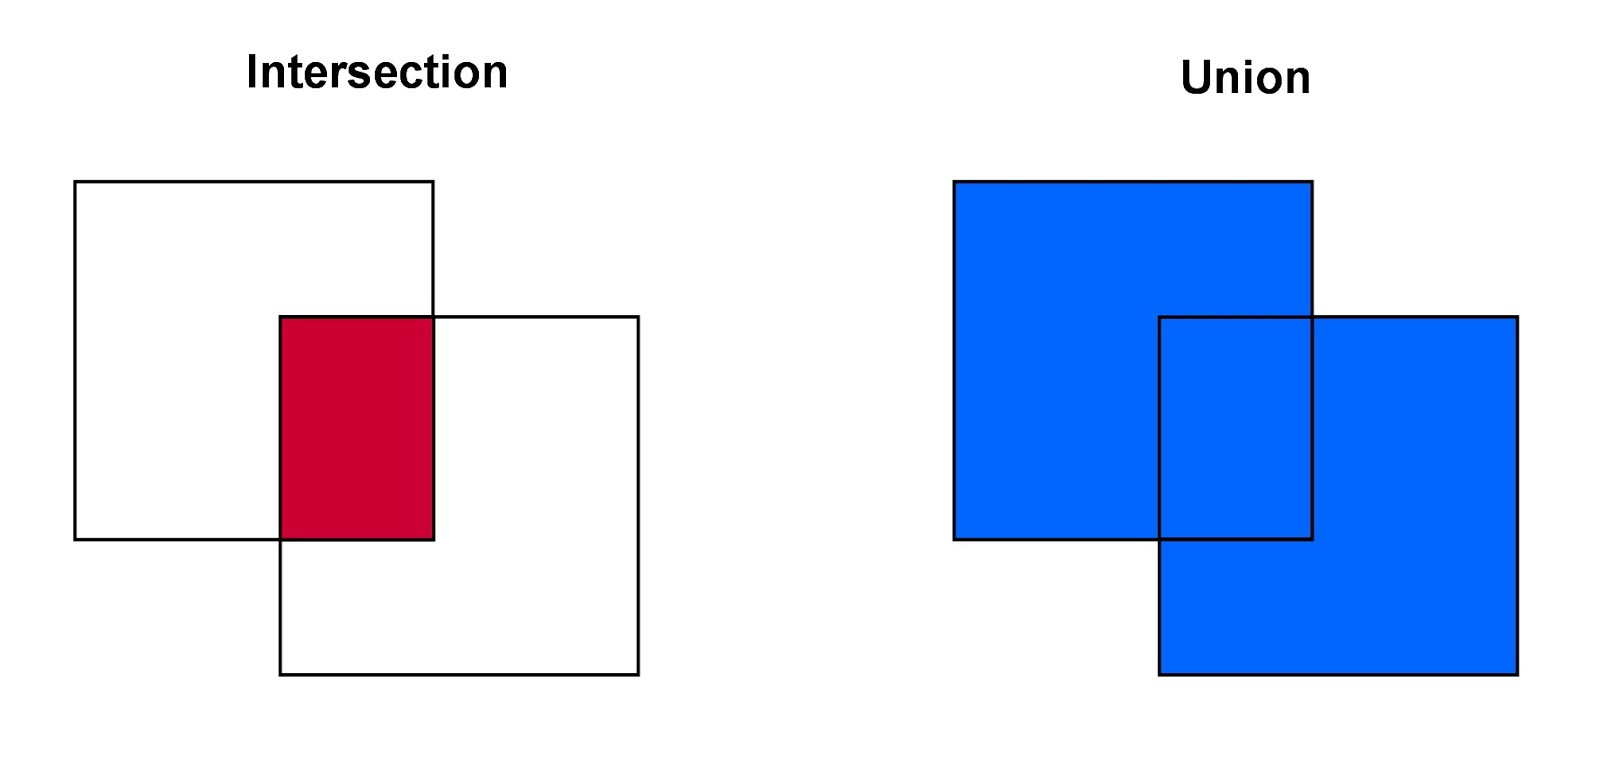
\includegraphics[width=0.5\linewidth]{images/unione-intersezione.jpg}
	\caption{Esempio di intersezione e di unione}
	\label{Esempio di intersezione e di unione}
\end{figure}
\subsubsection{Average Precision}
Una delle due metriche utilizzate è l'average precision (AP) e per calcolarla si fa la media delle precisioni di undici diversi valori di recall equamente distribuiti. Questa metrica viene applicata ad una sola categoria di elementi e viene calcolata tramite la seguente formula:
\[
    AP = \frac{1}{11}\sum_{Recall\ped{i}}^{} Precision(Recall\ped{i})
\]
Dove \textit{i}=[0, 0.1, 0.2, …, 1.0] in quanto 0 \textless  recall\textless 1. Inoltre la precisione di uno specifico valore di recall viene calcolata nel seguente modo:
\[
    Precision(Recall\ped{i}) = max\,Precision(Recall\ped{j}) \quad \textrm{and} \quad j>=i
\]
L'AP è un valore che riassume la forma della curva precision/recall per una data categoria.
\subsubsection{Mean Average Precision}
La mean average precision (mAP) è la media delle AP di tutte le categorie calcolata su diverse soglie di IoU:
\[
    mAP\ped{IoU=x\%} = \frac{1}{n}\sum_{i=0}^{n}AP\ped{i}
\]
Dove \textit{i} è il numero totale di categorie sulle quali è stata calcolata la propria AP e \textit{x} rappresenta diverse soglie di IoU.




